\section{Interpolation\label{ch:interpolation}}
Aufgabenstellung: Aus einer festgelegten Menge von Funktionen $M_n$ 
bestimme man eine Funktion, die durch die gegebenen Punkte
$(x_0, f_0), (x_1, f_1), \ldots, (x_n, f_n) \in \mathbb{R}^2$ verläuft.

\begin{figure}[htbp]
  \centering
  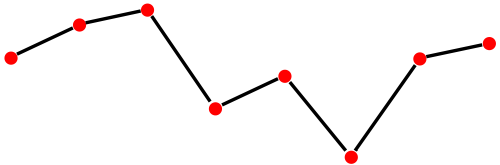
\includegraphics[width=0.7\textwidth]{figures/interpolation.png}
  \caption{Interpolation: Stützstellen sind in rot markiert}
  \label{fig:interpolation}
\end{figure}

Die Wahl von $M_n$ ist abhängig von der Problemstellung:
\begin{itemize}
  \item $\Pi_n$: Menge der Polynome mit Grad $\leq$ n
  \item stückweise polynomiale Funktion
  \item trigonometrische Funktion
	\item $\ldots$
\end{itemize}
Warum und weshalb:
\begin{itemize}
  \item Berechnung von Zwischenwerten einer Funktion, die nur an wenigen 
    Stellen bekannt ist
  \item Vereinfachung der Komplexität einer Funktion. (Beschreibung
    einer Funktion durch eine kleine Anzahl von Funktionen) $\Rightarrow$
    einfacheres Rechnen
  \item wichtige theoretische Grundlage für verschiedene andere numerische
    Aufgaben (Integration, Differenzialgleichungen)
\end{itemize}

\subsection{Polynominterpolation}
\underline{Gegeben}: Paarweise verschiedene Stützstellen $x_0, x_1, \ldots x_n$ und
Werte $f_0, f_1, \ldots f_n$.\\
\underline{Gesucht}:
\begin{equation*}
  \tag{2.1} p_n \in  \Pi_n \text{, so dass } p_n(x_i) = 
  f_i \text{ für } i = 0, 1, \ldots ,n
\end{equation*}
Grundlegende Fakten zu Polynomen:
\begin{enumerate}[(i)]
  \item $\Pi_n$ die Menge der Polynome mit Grad $\leq$ n ist ein Vektorraum
  \item Die Monome $1, x, x^2, \ldots, x^n$ bilden eine Basis von $\Pi_n$
  \item Polynom von Grad n $\geq$ 1 mit komplexen Koeffzienten besitzt genau n-Nullstellen
    in $\mathbb{C}$, wobei die Anzahl der Nullstellen entsprechend der Vielfachheit
    gezählt wird.
\end{enumerate}
\para{Satz} Die Polynominterpolationsaufgabe (2.1) ist eindeutig lösbar\\
Beweis:
\begin{enumerate}[(a)]
  \item Eindeutigkeit: Angenommen $p_n, q_n \in \Pi_n$ erfüllen (2.1), d.h. $p_n(x_i)=q_n(x_i)=f_i $ für $i=0,1,\ldots,n$\\
    $r := p_n - q_n \in \Pi_n$ \\
    $r(x_i) = 0$ für $i = 0, \ldots, n \Rightarrow r$ hat $n + 1$ Nullstellen
    $\Rightarrow r \equiv 0 \Rightarrow p_n \equiv q_n$
  \item Existenz: Konstruiere Polynome $L_0(x), L_1(x), \ldots, L_n(x) \in \Pi_n$ mit\\
    $L_i(x_k)=\begin{cases} 1 & \mbox{für } \mbox{ $i = k$} \\ 
      0 & \mbox{sonst} \end{cases}$ \\
    $\Rightarrow L_i$ hat n Nullstellen: $x_0, x_1, \ldots, x_{i-1}, x_{i+1}, \ldots, x_n$
		\begin{align*}    
		L_i \in \Pi_n \Rightarrow L_i(x) = a(x-x_0)(x-x_1)\ldots(x-x_{i-1})(x-x_{i+1})\ldots(x-x_n)\\
    L_i(x_i) \mustbe 1 \Rightarrow
      a = \frac{1}{(x_i-x_0)(x_i-x_1)\ldots(x_i-x_{i-1})(x_i-x_{i+1})\ldots(x_i-x_n)}\\
    \end{align*}
		\begin{empheq}[innerbox=\fbox,right=\Leftarrow{\text{LAGRANGE-POLYNOME}}]{align*}
		\Rightarrow L_i(x) = \frac{(x - x_0)\ldots}{(x_i - x_0)\ldots} = 
      \prod\limits_{j = 0,\,j \neq i}^n \frac{x - x_j}{x_i - x_j} \\
		\end{empheq}
    \begin{equation*}
      \tag{2.2}
      p_n(x) = f_0 L_0(x) + f_1 L_1(x) + \ldots + f_n L_n(x) = 
      \sum\limits_{k = 0}^n f_k L_k(x)
    \end{equation*}
    $p_n(x_i) = 0 + 0 + \ldots + f_i\underbrace{L_i(x_i)}_{1} + 0 + \ldots = f_i$\\
\end{enumerate}

% 17.10.2012
%Wh. Polynominterpolation

%\begin{align*}
%\text{geg.} \hspace{0.5cm} & (x_0,f_0),\ldots\,,(x_n,f_n) \\
%\text{ges.} \hspace{0.5cm} & p_n \in \Pi_n:p_n(x_i)=f_i & \Rightarrow p_n(x) = f_0\,L_0+\ldots\,+f_n\,L_n(x) \hspace{1cm} (2.2)\\
%& & L_i(x)=\prod\limits_{i=0,i\neq\,j}^n \frac{x-x_j}{x_i-x_j}
%\end{align*}

%\begin{equation*} 
  %L_i(x_k)
	%\left\{  
  %\begin{aligned} 
   %& i=k: 1 \\ 
   %& i\neq\,k: 0\\
  %\end{aligned} 
	%\right.
%\end{equation*} 

(2.2) nennt man Lagrange-Darstellung des Interpolationspolynoms (IP) [theoretisch von Interesse]

\subsubsection{Effiziente Berechnung und Auswertung des IPs (Newton-Darstellung)}
\underline{Nachteile der Lagrange-Darstellung:}

\begin{itemize}
	\item Hinzunahme neuer Daten ($x_{n+1},f_{n+1}) \Rightarrow$ komplett neue Berechnung notwendig
	\item Auswertung des IPs ist nicht effizient $L_i$
\end{itemize}

\para{Definition}
Zu $x_0,\ldots,x_n$ sind die Newton-Basispolynome definiert durch:

\begin{align*}
&N_0 \equiv 1\\
&N_1(x) = (x-x_0)\\
&N_2(x) = (x-x_0)(x-x_1)=N_1(x)(x-x_1)\\
&\vdots \\
&N_n(x) = (x-x_0)(x-x_1)\ldots\,(x-x_{n-1})=N_{n-1}(x)(x-x_{n-1})
\end{align*}
$N_0,\ldots\,,N_n$ bilden eine Basis von $\Pi_n$ (lässt sich einfach zeigen).\\
Ansatz: für Polynominterpolation $(x_0,f_0)\ldots\,(x_n,f_n)$:\\
Suche: $a_0,\ldots\,,a_n$ so dass 

\begin{align*}
p_n(x)&=a_0\,N_0(x) + \ldots\, + a_n\,N_n(x) \quad \text{und} \\
p_n(x_i)&= f_i \quad \text{für} \quad i=0\ldots\,n \\
f_0 &\mustbe p_n(x_0) = a_0\,\underbrace{N_0(x_0)}_{1} + \underbrace{a_1\,\underbrace{N_1(x_0)}_{(x_0-x_0)} + \ldots + a_n\,N_n(x_0)}_{=0} \\
& \Rightarrow a_0 = f_0 \\
f_1 &\mustbe p_n(x_1) = a_0\cdot\,1 + a_1\,(x_1-x_0) + \underbrace{a_2\,(x_1-x_0)(x_1-x_1)}_{=0} + 0  \\
& a_1 = \frac{f_1-a_0}{x_1-x_0}\\
f_n &\mustbe p_n(x_n) = a_0\,N_0(x_n) + \ldots + a_n\,N_n(x_n) \\
& a_0,\ldots\,,a_n \quad \text{lassen sich durch Vorwärtseinsetzen bestimmen}
\end{align*}\\

\underline{Effizienter Algorithmus:} Dividierte Differenzen
\para{Definition}
Zu $(x_0,f_0),\ldots\,,(x_n,f_n)$ mit $x_i\neq\,x_j$ für $i\neq\,j$ sind die div. Differenzen definiert durch
\begin{align*}
f[x_i] &= f_i \quad i=0\ldots\,n\\
f[x_i,x_{i+1},\ldots\,,x_{i+m}] &:= \frac{f[x_{i+1},\ldots\,,x_{i+m}]-f[x_{i},\ldots\,,x_{i+m-1}]}{x_{i+m}-x_i}
\end{align*}

\para{Satz}
Sei $p_n\in\,\Pi_n$ das IP zu $(x_0,f_0)\ldots\,(x_n,f_n)$ dann gilt:
\begin{equation*}
p_n(x) = f[x_0]\,N_0(x)+f[x_0,x_1]\,N_1(x)+\ldots\,+f[x_0,x_n]\,N_n(x)
\end{equation*}
Beweis erfordert mehr als "`Einsetzen"'. \\
\underline{Schema zur Berechnung:}

\begin{tabular}{c|l}
$x_0$ & $f_0 = f[x_0] \searrow$ \\
$x_1$ & $f_1 = f[x_1] \rightarrow f[x_0,x_1]  \searrow$ \\
$x_2$ & $f_2 = f[x_2] \rightarrow f[x_1,x_2] \rightarrow f[x_0,x_1,x_2]$\\
$\vdots$ &  \\
$x_{n-1}$ & $f_{n-1} = f[x_{n-1}] \rightarrow \ldots \rightarrow f[x_0,\ldots\,,x_{n-1}] \searrow$\\
$x_n$ & $f_n = f[x_n] \rightarrow \ldots \rightarrow f[x_1,\ldots\,,x_n] \rightarrow f[x_0,\ldots\,,x_n]$ \\
\end{tabular}

\para{Einschub: Vollständige Induktion (Beweistechnik)}
Um zu beweisen, dass Aussage A für alle natürlichen Zahlen $n\geq\,n_0$ gilt, reicht es zu zeigen:

\begin{enumerate}
	\item A gilt für $n_0$ [Induktionsanfang, IA] 
	\item Aus der Gültigkeit von A für eine Zahl $n$, folgt eine Gültigkeit von A für $n+1$ [Induktionsschritt, $A(n)\Rightarrow A(n+1)$, IS]
\end{enumerate}

Beispiel: Gauß'sche Summenformel\\
$\sum\limits_{i=1}^{n}{i}=?$\\\\
a) Gauß Lösung\\
\begin{center}
\begin{tabular}{c|c|c|c|c}
	1 & 2 & 3 & $\ldots$ & n \\
	n & n-1 & n-2 & $\ldots$ & 1 \\\hline
  n+1 & n+1 & n+1 & $\ldots$ & n+1
\end{tabular}
$\Rightarrow\,\sum\limits_{i=1}^{n}{i}=\frac{n}{2}(n+1)$ (*)\\
\end{center}
b) Vollständige Induktion

\begin{enumerate}
	\item IA $n_0=1$ $\sum\limits_{i=1}^{n=1}{i}=1\mustbe\,\frac{1}{2}(1+1)=1 \Rightarrow ok$
	\item IS $n \mapsto n+1$ Annahme (*) gilt für n. Zu zeigen: (*) gilt für n+1, d.h. z.z.\\
	$\sum\limits_{i=1}^{n+1}{i}=\frac{1}{2}(n+1)(n+1+1)=\frac{n^2+3n+2}{2}$\\
	$\sum\limits_{i=1}^{n+1}{i}=\underbrace{\sum\limits_{i=1}^{n}{i}}_{Annahme} + n+1$ \\
	$=\frac{n}{2}(n+1) + \frac{2(n+1)}{2}= \frac{n^2+3n+2}{2} \Rightarrow ok$
\end{enumerate}

\para{Behauptung}
Die Berechnung von $f[x_0], f[x_0,x_1],\ldots,f[x_0,\ldots\,,x_n]$ benötigt $\frac{3n(n+1)}{2}$ Flops. \\
Beweis: Vollständige Induktion\\

\begin{enumerate}
	\item IA, $n_0=1 \quad f[x_0],f[x_0,x_1]=\frac{f[x_1]-f[x_0]}{x_1-x_0} \Rightarrow 3 \mustbe \frac{3\cdot\,1(2)}{2}=3 \Rightarrow ok$
	\item IS $n \mapsto n+1 \quad$ Annahme: Aufwand für $f[x_0], \ldots\,f[x_0,\ldots\,,x_n]$ beträgt $\frac{3n(n+1)}{2}$ Flops. Z.z. für $\underbrace{f[x_0], \ldots\,,f[x_0,\ldots\,,x_n]}_{\text{wissen wir}},f[x_0,\ldots,x_{n+1}]$ sind $\frac{3(n+1)(n+1+1)}{2}$ Flops nötig. \\
Aufwand für $f[x_0,\ldots\,,x_{n+1}]$\\
\begin{tabular}{c|l}
\vdots \\
$x_{n}$ & $f_{n} = f[x_{n}] \searrow$\\
$x_{n+1}$ & $f_{n+1} = f[x_{n+1}] \rightarrow \underbrace{f[x_n,x_{n+1}] \rightarrow f[x_{n-1},x_n,x_{n+1}] \rightarrow f[x_0,\ldots\,,x_{n+1}]}_{\underbrace{\text{n+1 d.D. mit jeweils 3 Flops}}_{3(n+1)}}$ 
\end{tabular}

D.h. insgesamt $\underbrace{f[x_0],\ldots\,,f[x_0,\ldots\,,x_n]}_{\frac{3n(n+1)}{2}} + \underbrace{f[x_0,\ldots\,,x_{n+1}]}_{\frac{2\cdot\,3n(n+1)}{2}} = \frac{(n+2)3(n+1)}{2} \Rightarrow $ ok
\end{enumerate}

\para{2.1.1.1 Horner Schema (Auswertung von Polynomen)}
Naive Auswertung von $p_n(x) = a_0+a_1x+\ldots\,+a_nx^n$ erfordert 

\begin{itemize}
	\item $x^2, x^3,\ldots\,,x^n \rightarrow$ n-1 Multiplikationen
	\item $a_i\cdot\,x^i \quad i = 1\ldots\,n \rightarrow$ n Mulitplikationen
	\item n Additionen
\end{itemize}

\underline{Horner Schema}
$p_n(x) = a_0 + x\cdot\,(a_1 + x\cdot\,(a_2 + \ldots + x\cdot\,(\underbrace{a_{n-2} + x\cdot\,(\underbrace{a_{n-1} + x\cdot\,(a_n))}_{b_{n-1}}}_{b_{n-2}}\ldots\,)$
Auswertung von innen nach außen:

\begin{equation*}
\left.
\begin{aligned}
 b_n &:= a_n \\
 b_{n-1} &:= a_{n-1} + x\,b_n \\
 b_{n-2} &:= a_{n-2} + x\,b_{n-1} \\
 & \vdots \\
 b_{1} &:= a_{1} + x\,b_{2} \\
 b_{0} &:= a_{0} + x\,b_{1} 
\end{aligned}
\right\}
\text{Aufwand: } \\
\text{n Multiplikationen, n Additionen}
\end{equation*}
$\Rightarrow p_n(x) = b_0$\\

Horner Schema zur Auswertung von $p_n$ in Newtondarstellung:\\
\begin{align*}
 p_n(x) &= \underbrace{f[x_0]}_{a_0}\underbrace{N_0(x)}_{1} + \underbrace{f[x_0,x_1]}_{a_1}\underbrace{N_1(x)}_{(x-x_0)}
+ \underbrace{f[x_0,x_1,x_2]}_{a_2}\underbrace{N_2(x)}_{(x-x_0)(x-x_1)} + \ldots + \underbrace{f[x_0,\ldots\,,x_n]}_{a_n}\underbrace{N_n(x)}_{(x-x_0)\ldots(x-x_n)} \\
 &= a_0 + (x-x_0)(a_1 + (x-x_1)(a_2+ \ldots + (x-x_{n-2})(a_{n-1})+(x-x_{n-1})(a_n))\ldots)) \\
\end{align*}
\begin{equation*}
\left.
\begin{aligned}
 b_n &:= a_n \\
 b_{n-1} &:= a_{n-1} + (x-x_{n-1})b_n \\
 b_{n-2} &:= a_{n-2} + (x-x_{n-2})b_{n-1} \\
 \vdots \\
 b_0 &:= a_0 + (x-x_0)b_1
\end{aligned}
\right\}
\text{Aufwand: }
\text{2n Additionen, n Multiplikationen}
\end{equation*}

\subsubsection{Absolute Kondition der Polynominterpolation}
Geg.: Exakte Daten $(x_0, f_0), \ldots, (x_n, f_n)$ wobei $x_0, \ldots, x_n \in [a, b]$ und
gestörte Daten $(x_0, f_0 + \Delta_0), \ldots, (x_n, f_n + \Delta_n)$ \\
Ges.: Maximale Abweichung der Interpolationspolynome $p_n(x) = \sumizn{f_i L_i(x)}$ und
$p^{\Delta}_n(x) = \sumizn{(f_i + \Delta_i) L_i(x)}$ im Intervall $[a, b]$ \\
WH:
\begin{align*}
  \maxxab \abs{\alpha f(x) + \beta g(x)} &\leq
    \maxxab \abs{\alpha} \abs{f(x)} + \maxxab \abs{\beta} \abs{g(x)} \\
  &\leq \max\{\abs{\alpha}, \abs{\beta}\}\, \maxxab\{\abs{f(x)}, \abs{g(x)}\}
\end{align*}

\begin{align*}
  \maxxab \abs{p_n(x) - p^{\Delta}_n(x)} = \maxxab \sumizn{\abs{\Delta_i L_i(x)} } \leq
  \underset{0 \leq i \leq n}{\max}\,\abs{\Delta_i} \maxxab \sumizn{\underbrace{\abs{L_i(x)}}_{\geq 1}}
\end{align*}
Maß für dier Verstärkung des Eingangsfehlers:
\begin{equation*}
  \maxxab \sumizn{\abs{L_i(x)}} =: \Lambda_n(x_0, \dots, x_n) = \Lambda_n 
  \text{ Lebesque Konstante}
\end{equation*}
Ändert sich nicht durch affin-lineare Transformation der Stützstellen.
\example{Bsp:} Interpolation von $f(x) =\sin(2\pi x)$ in $[-1, 1]$ mit 21
gleichverteilten Stützstellen. $p_{20}, p_{20}^\Delta$ mit Störung $\Delta_9 = -10^{-3}$
\begin{figure}[htbp]
  \centering
  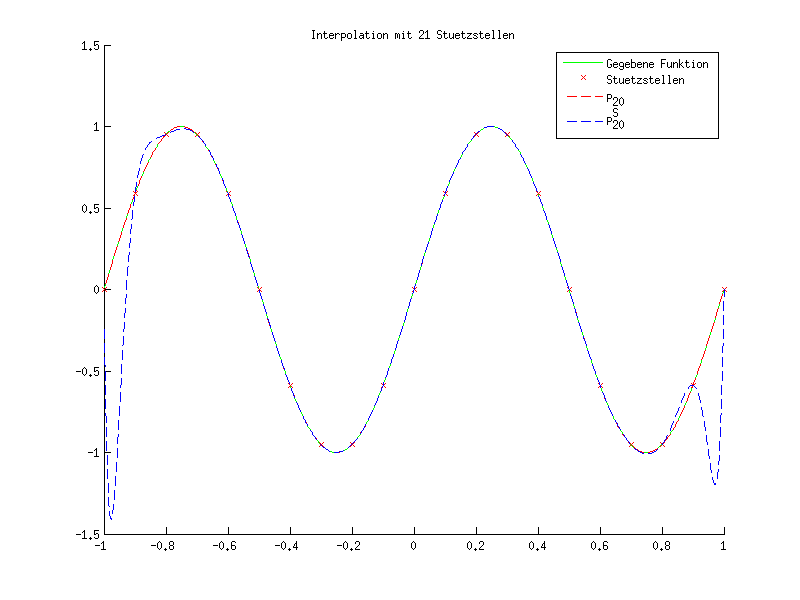
\includegraphics[width=\textwidth]{figures/interpolation_stoerung.png}
  \caption{Interpolation mit und ohne Störung.}
  \label{fig:interpolation-stoerung}
\end{figure}

\subsubsection{Fehlerschätzung der Polynominterpolation}
\para{Satz}
Sei $f \in C^{n+1} [a, b]$ ($(n+1)$ mal stetig differenzierbar) und $p_n \in \Pi_n$
das Interpolationspolynom in den paarweise verschiedenen Stützstellen $x_0, \dots, x_n$
interpoliert, dann existiert für jedes $x \in [a, b]$ ein $\zeta \in [a, b]$ so, dass
\begin{align*}
  f(x) - p_n(x) = \frac{1}{(1 + n)!} f^{(n+1)}(\zeta(x))(x - x_0)\cdot \dots \cdot(x - x_n)
\end{align*}
Ist $f \in C^\infty [a, b]$ und gelte $\maxxab \abs{f^{(n)}(x)} \leq M \, \forall n \in \mathbb{N}$ \\
\begin{align*}
  \Rightarrow \maxxab \abs{f(x) - p_n(x)} \leq 
  \frac{1}{(1 + n)!}M(b - a)^{n + 1} \xrightarrow[x\to\,\infty]{} 0
\end{align*}

%TODO define a \subsubsubsction?
\para{Tschebyscheff Interpolation}
Maximale Fehler der Polynominterpolation einer Funktion f ist abhängig von f und ihren
Ableitungen sowie der Wahl der Stützstellen, d.h. vom Term
$(x - x_0)\cdot \ldots \cdot(x - x_n)$. \\
Idee: Wähle $x_0, \ldots, x_n$ so, dass $\maxxab \abs{(x - x_0)\cdot \ldots \cdot(x - x_n)}$
minimal ist. \\
$\Rightarrow$ Minmax-Aufgabe \\
Zunächst: Spezieller Fall $[a, b] = [-1, 1]$. Danach Übertragung auf allgemeins
Intervall. \\
Definition: Die Tschebyscheff-Polynome sind definiert durch
\begin{align*}
  T_o(x) &\equiv 1\\
  T_1(x) &= x\\
  T_n(x) &= 2xT_{n-1}(x) - T_{n-2}(x)\,\, n = 2, 3, \ldots
\end{align*}
Im Intervall $[-1, 1]:\,T_n(x) = \cos(n\arccos(x))$ (Beweis über Additoinstheoreme)
\para{Satz} Für die Nullstellen des Tschebyscheff-Polynoms $T_{n+1}$, 
$\overline{x}_i^{(n+1)} = \cos(\frac{2i + 2}{2(n + 1)}\pi)\, i = 0, \ldots, n$ gilt:
\begin{align*}
  \underset{x_0, \ldots, x_n \in [a, b]}{min} \, \maxxab |(x - x_0)
    \cdot \ldots \cdot(x - x_n)| = 
    \maxxab |(x - \overline{x}_0^{(n + 1)})\cdot \ldots 
    \cdot(x - \overline{x}_n^{(n + 1)})| =\frac{1}{2^n}
\end{align*}
Fehlerabschätzung für 
$\overline{x}_0^{(n + 1)}\cdot \ldots \cdot\overline{x}_n^{(n + 1)}$: 
$\maxmpo\abs{f(x) - p_n(x)} \leq \frac{1}{(n + 1)!} \maxmpo \abs{f^{(n + 1)}} \frac{1}{2^n}$ \\
Allgemeiner Fall $[a, b]$: Verwende affin-lineare Transformation für die Stützstellen \\
$\overline{x}_0^{(n + 1)}\cdot \ldots \cdot\overline{x}_n^{(n + 1)}$:
\begin{align*}
  \psi: [-1, 1] &\longrightarrow [a, b] \\
  x &\longmapsto \frac{1}{2}((b - a)x + a + b) \\
  \psi(-1) = a\,\,&\,\, \psi(1) = b
\end{align*}
Es gilt $\psi(\overline{x}_0^{(n + 1)}),\,\ldots,\,\psi(\overline{x}_n^{(n + 1)})$ ist
Lösung der Minmax-Aufgabe.

% 2.1.3.2
\para{Indikator für die Güte der Wahl der Stützstellen}
Wie gut ist für eine Funktion f die Polynominterpolation für eine bestimmte Wahl
von $n + 1$ Stützstellen im Vergleich zur bestmöglichen Approximation der Funktion f
durch ein Polynom?
\para{Satz} Sei $f:[a, b] \longrightarrow \mathbb{R}$ stetig.
\begin{enumerate}[(a)]
  \item Es gibt eine Folge von Polynomen $(q_n)$ mit $q_n \in \Pi_n$, so dass
    \begin{equation*}
      \maxxab \abs{q_n(x) - f(x)} \underset{n \to \infty}{\longrightarrow} 0
    \end{equation*}
  \item Es existiert genau eine Bestapproximation $q_n^* \in \Pi_n$ mit
    \begin{equation}
      \tag{2.3}
      \maxxab \abs{q_n^*(x) - f(x)} \leq \maxxab \abs{p(x) - f(x)} \; \forall p \in \Pi_n
    \end{equation}
\end{enumerate}
\para{Satz} Sei $f:[a, b] \longrightarrow \mathbb{R}$ stetig. $\xztoxn$
seien paarweise verschiedene Stützstellen in $[a, b]$. Für $q_n^* \in \Pi_n$ gelte
(2.3). Für das Interpolationspolynom $p_n \in \Pi_n$, das f in den Stützstellen
$\xztoxn$ interpoliert gilt:
\begin{equation*}
  \maxxab \abs{p_n(x) - f(x)} \leq (1 + \Lambda_n(\xztoxn))\,\maxxab \abs{q_n^*(x) - f(x)}
\end{equation*}
\para{Beweis}
\begin{align*}
  \maxxab \abs{p_n(x) - f(x)} &= \maxxab \abs{p_n(x) - q_n^*(x) + q_n^*(x) - f(x)}\\
  &\leq \maxxab \abs{p_n(x) - q_n^*(x)} + \underbrace{\maxxab \abs{q_n^*(x) - f(x)}}_{=:A}\\
  &= \maxxab \abs{\sumizn[f(x_i) - q_n^*(x_i)]L_i(x)} + A\\
  &\leq \underbrace{\maxxab \abs{f(x) - q_n^*(x)}}_A \: \underbrace{ \maxxab \sumizn{\abs{ L_{i}(x) }} + A}_{\Lambda_n} \\
  &= (1 + \Lambda_n) \: \maxxab \abs{f(x) - q_n^*(x)}
\end{align*}
\begin{figure}[htbp]
  \centering
  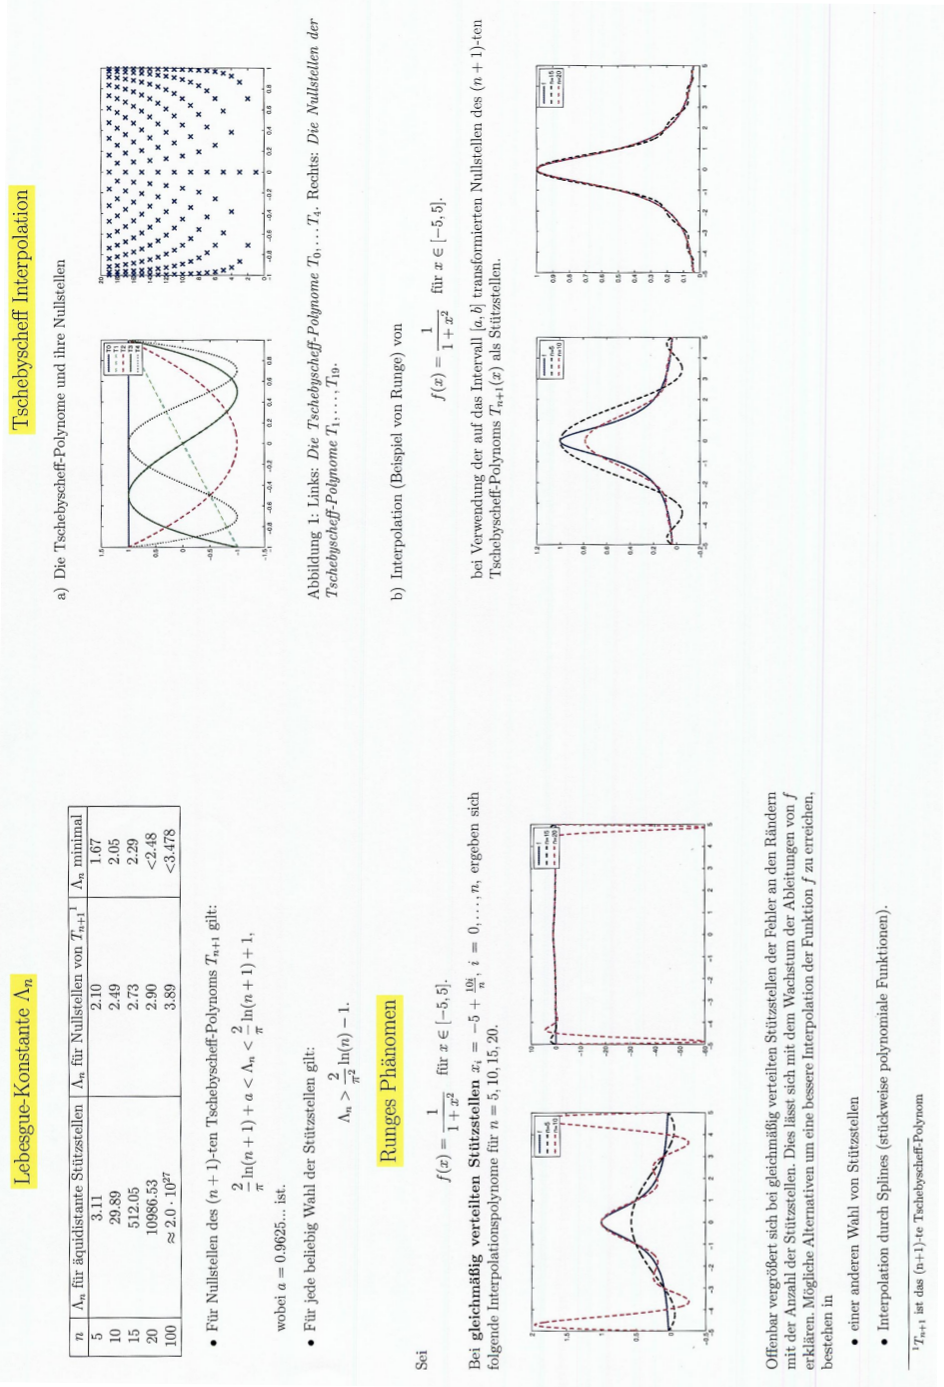
\includegraphics[width=\textwidth]{figures/handout_interpolation.png}
\end{figure}
\subsection{Stückweise polynomiale Interpolation}
Die Interpolation einer Funktion $f:[a,b] \longrightarrow \mathbb{R}$ durch Polynome hohen Grades
kann aus verschiedenen Gründen problematisch sein (Prüfungsfrage: wo ist es nicht problematisch):
\begin{itemize}
  \item Fehlerschranken erfordern hohe Differenzierbarkeit von f
  \item Konvergenzgeschwindigkeit $f-p_n$ für $n \rightarrow \infty$ ist unbefriedigend
  \item Polynome hohen Grades können stark oszillieren (z.B.: grafische Anwendung $\leftarrow$ unerwünscht)
\end{itemize}

Alternativer Ansatz: Anstatt den Polynomgrad zu erhöhen, unterteile zuerst $[a,b]$ in Teilintervalle
$\rightarrow$ Polynominterpolation niedriger Ordnung

\subsubsection{Stückweise lineare Interpolation}
Beispiel: siehe Abbildung~\ref{fig:interpolation}
\para{Definition:}
Sei $[a,b] \subset \mathbb{R}$ und $a=x_0<\ldots<x_n=b$ eine Unterteilung von $[a,b]$, dann bezeichnet
\begin{align*}
  S_L:=\{s_L:s_L\in C[a,b] \text{ und } s_L \text{ ist linear in } [x_{i-1},x_i],\,i=1,\ldots,n\}
\end{align*}
den Raum der stückweise linearen Funktionen bezüglich der Unterteilung $x_0,\ldots,x_n$.
(S steht für Spline und L bedeutet dass es sich um ein lineares Spline handelt.)\\
Basis?\\
\para{Definition:}
Sein $[a,b] \subset \mathbb{R}$ und $a=x_0<\ldots<x_n=b$. Die Hutfunktionen $\phi_0,\ldots,\phi_n$
sind folgendermaßen definiert:
\begin{align*}
  \phi_{k=1,\ldots,n-1}(x) &= \begin{cases}
    \frac{x-x_k{k-1}}{x_k-x_{k-1}} &\mbox{für } x\in[x_{k-1},x_k]\\
    \frac{x_{k+1}-x}{x_{k+1}-x_k} &\mbox{für } x\in[x_k,x_{k+1}]\\
    0 &\mbox{sonst}
  \end{cases}\\
  \phi_0(x) &= \begin{cases}
    \frac{x_1-x}{x_1-x_0} &\mbox{für } x\in[x_0,x_1]\\
    0 &\mbox{sonst}
  \end{cases}\\
  \phi_n(x) &= \begin{cases}
    \frac{x-x_{n-1}}{x_n-x_{n-1}} &\mbox{für } x\in[x_{n-1},x_n]\\
    0 &\mbox{sonst}
  \end{cases}
\end{align*}
\begin{figure}[htbp]
  \centering
  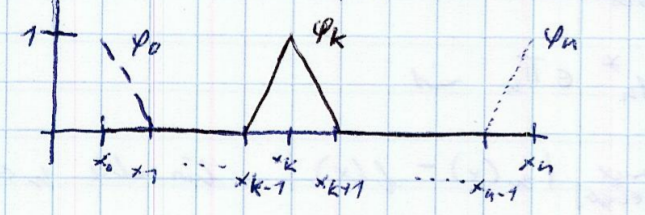
\includegraphics[width=0.7\textwidth]{figures/hutfunktionen.png}
  \caption{Hutfunktionen}
\end{figure}
Man beachte:
\begin{align*}
  \phi_i(x_j) = \begin{cases}
    1 &\mbox{für } i=j\\
    0 &\mbox{für } i \neq j
  \end{cases}
\end{align*}
Vorteil bei Verwendung von Hutfunktionen: Einfache Darstellung der stückweise
linearen Interpolationsfunktion $s_L$ zu $(x_0,f_0),\ldots,(x_n,f_n)$:
\begin{align*}
  s_L(x)=\sum_{i=0}^n f_i \phi_i(x) \text{, denn } s_L(x_k)=\sum_{i=0}^n f_i \phi_i(x_k) = f_k \underbrace{\phi_k(x_k)}_{1} = f_k
\end{align*}
\para{Satz:} Sei $f \in C^n[a,b]$ und $s_L$ die stückweise lineare Funktion, die f in den Knoten
$a=x_0<\ldots<x_n=b$ interpoliert. Dann gilt:
\begin{align*}
  \maxxab \abs{f(x)-s_L(x)} \leq \frac{1}{8}h_{max} \maxxab \abs{f''(x)}
\end{align*}
wobei $h_{max} = \underset{1 \leq i \leq n}{\max} \underbrace{x_i - x_{i-1}}_{=:h_i}$
\para{Beweis:} Betrachte $[x_{i-1},x_i]$:
\begin{figure}[htbp]
  \centering
  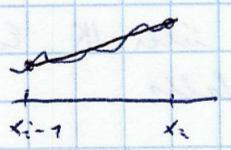
\includegraphics[width=0.3\textwidth]{figures/zwischenstuetzstellen.png}
  \caption{Möglicher Verlauf zwischen Stützstellen}
\end{figure}
Fehlerdarstellung für Polynominterpolation in $[x_{i-1},x_i]$:
\begin{align*}
  f(x)-s_L(x) &= \frac{1}{2!} f''(\xi(x))(x-x_{i-1})(x-x_i) \,\, \xi(x) \in [x_{i-1},x_i]\\
  \abs{f(x)-s_L(x)} &\leq \frac{1}{2} \underset{\xi(x) \in [x_{i-1},x_i]}{\max}\abs{f''(\xi)} 
  \underbrace{\underset{x \in [x_{i-1},x_i]}{\max}\abs{(x-x_{i-1})(x-x_i)}}_{\frac{h_i}{2}\cdot\frac{h_i}{2}\leq\frac{1}{4}h_{max}^2}\\
  &\leq \frac{1}{8} \underset{\xi(x) \in [x_{i-1},x_i]}{\max}\abs{f''(\xi)} h_{max}^2\\
  &\leq \frac{1}{8} \underset{\xi(x) \in [a,b]}{\max}\abs{f''(\xi)} h_{max}^2\\
\end{align*}
\begin{figure}[htbp]
  \centering
  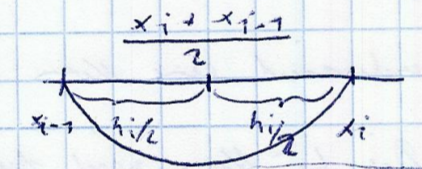
\includegraphics[width=0.3\textwidth]{figures/fehler_letzter_teil.png}
  \caption{Darstellung des letzten Fehlerterms $(x-x_{i-1})(x-x_i)$}
\end{figure}
\para{Einschub: Norm und Skalarprodukt}
Norm dient als Maß um Fehler bzw. Genaugigkeit zu messen.\\
\para{Definition:} Sei $V$ ein Vektorraum über $\mathbb{K}\,(\mathbb{K}=\mathbb{R}, \mathbb{K}=\mathbb{C})$.
Eine Abbildung $\norm{.}: V\rightarrow\mathbb{K}$ heißt Norm auf $V$, falls
\begin{itemize}
  \item $\norm{v}>0\, \forall\, v \in V$ und aus $\norm{v}=0 \Rightarrow v = 0$
  \item $\norm{\alpha v} = \abs{\alpha}\,\norm{v}\, \forall\, \alpha \in \mathbb{K}\, \forall\, v \in V$
  \item $\norm{v+w} \leq \norm{v} + \norm{w}\, \forall\,v,w\in V$
\end{itemize}
Beispiel: $V=\mathbb{R}^n$\\
\begin{itemize}
  \item $\norm{v}_2 = \sqrt{\sumion{[v_i]^2}}$ (Euklidische Norm)
  \item $\norm{v}_{\infty} = \underset{1 \leq i \leq n}{\max} \abs{v_i}$ (Maximumsnorm)
\end{itemize}
Beispiel: $V=C[a,b]$
\begin{itemize}
  \item $\norm{f}_{L2(a,b)} = \sqrt{\int_a^b \abs{f(x)}^2 \dx}$ (L2-Norm)
  \item $\norm{f}_{\infty} = \maxxab \abs{f(x)}$
\end{itemize}
In unendlich dimensionalen Räumen (z.B $C[a,b], L2[a,b]$) sind Normen
\large{\textcolor{rot}{\textbf{nicht}}} äquivalent, d.h. Konvergenz 
in $\norm{.}_1$ bedeutet nicht Konvergenz in $\norm{.}_2$.\\
Bemerkung: Der größtmögliche Raum auf dem die L2-Norm definiert ist, ist
\begin{align*}
  L2(a,b) := \{f:\norm{f}_{L2(a,b)} < \infty\}
\end{align*}
$L2(a,b)$ ist Obermenge von $C[a,b]$.
\para{Definition:} Sei $V$ ein Vektorraum über $\mathbb{K}$. Eine Abbildung $\inner{.}{.}:V \times V \rightarrow \mathbb{R}$
heißt Skalarprodukt, falls
\begin{itemize}
  \item $\inner{v}{v} \geq 0\, \forall\, v \in V$ und $\inner{v}{v}=0 \Leftrightarrow v=0$
  \item $\inner{v}{w} = \overline{\inner{w}{v}}$
  \item $\inner{\alpha v + \beta w}{z} = \alpha \inner{v}{z} + \beta \inner{w}{z} \, \forall\,v,w,z\in V$
\end{itemize}
Beispiel: $V=\mathbb{R}^n$ Euklidisches Skalarprodukt
\begin{align*}
  \inner{v}{w}_2 = \sumion v_i \cdot w_i
\end{align*}
\para{Satz:} Jedes Skalarprodukt induziert eine Norm durch
\begin{align*}
  \norm{v}=\sqrt{\inner{v}{v}}
\end{align*}
Beispiel: $V=L_2(a,b)$: Die L2-Norm wird durch das L2-Skalarprodukt induziert:
\begin{align*}
  \inner{f}{g}_{L2(a,b)} := \int_a^b f(x) \overline{g(x)} \dx
\end{align*}
Bemerkung: Es lässt sich zeigen, dass die Maximumsnorm
nicht durch ein Skalarprodukt induziert wird.
\para{Satz (Cauchy-Schwarzsche Ungleichung):} Sei $\inner{.}{.}$ ein Skalarprodukt in $V$
und $\norm{.}$ die induzierte Norm. Dann gilt:
\begin{align*}
  \abs{\inner{v}{w}} \leq \norm{v}\,\norm{w}\, \forall\, v,w \in V
\end{align*}
Beweis: Einsetzen, siehe Wikipedia.\\
Beispiel: $L2(a,b)$
\begin{align*}
  \abs{\int_a^b f(x)\overline{g(x)}\dx} \leq \sqrt{\int_a^b \abs{f(x)}^2 \dx}\sqrt{\int_a^b \abs{g(x)}^2 \dx}
\end{align*}
Unterschied zwischen $\norm{.}_{\infty}$ und $\norm{.}_{L2}$: Sei
\begin{align*}
  f:[a,b] & \longrightarrow \mathbb{R} \\
  t &\mapsto f(t) \text{ Verbrauch}
\end{align*}
\begin{figure}[htbp]
  \centering
  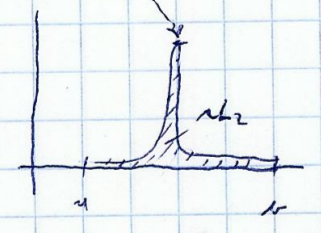
\includegraphics[width=0.3\textwidth]{figures/norms_l2_vs_infty.png}
  \caption{L2-Norm vs. $\infty$-Norm}
\end{figure}
L2-Norm als Maß für den ``Gesamtverbrauch''
